This section contains the results for the SSP5-8.5, the gradual SAI and the rapid cooling SAI experiments that are relevant for analysis of the upper stratosphere and the polar night jet (PNJ).

The potential temperature and zonal wind anomalies from section \ref{lowerstrat} showed the largest differences in the JJA mean, but the polar night jet is strongest in late winter and early spring. Al figures in this section will therefore consider the August-September-October (ASO) mean. 

\subsection{Polar Night Jet}
Figure \ref{fig:PNJ_UT_U_zmdiff} shows the zonal component of the thermal wind and the anomalies in Control, SAI 2020 and SAI 2080 in ASO. As in section \ref{lowerstrat} the observed wind and the thermal wind show the same patterns, with the thermal wind consistently higher than the observed wind due to friction effects. 

In control the PNJ shifts equatorward, with its strength not significantly changing. In SAI 2020 and SAI 2080 the PNJ shifts equatorward as well, but in contrast to Control the wind speed increases significantly. The pattern in SAI 2080 is the same as in SAI 2020, but the increase is much smaller. 

The kinetic energy per unit mass shown in Figure \ref{fig:PNJ_KE_U_zmdiff} shows largely the same pattern as the thermal wind in Figure \ref{fig:PNJ_UT_U_zmdiff}. In Figure \ref{fig:PNJ_EKE_U_zmdiff} the eddy kinetic energy is shown. In Control there is a decrease in EKE on the poleward side of the PNJ that is large relative to the KE decrease, indicating a relative deacrease in eddy activity.

The decrease in EKE over the Antarctic is visible in SAI 2020 and SAI 2080 as well, though lower, it still indicates a relative decrease in eddy activity. Where the KE increase is largest, the EKE increases the most as well, though contrastingly there is a second peak in EKE increase more equatorward, indicating an increase in eddy activity on the equatorward side of the PNJ. As with the KE, this increase is stronger in SAI 2020 than it is in SAI 2080. 

\begin{figure}[H]
	\centering
	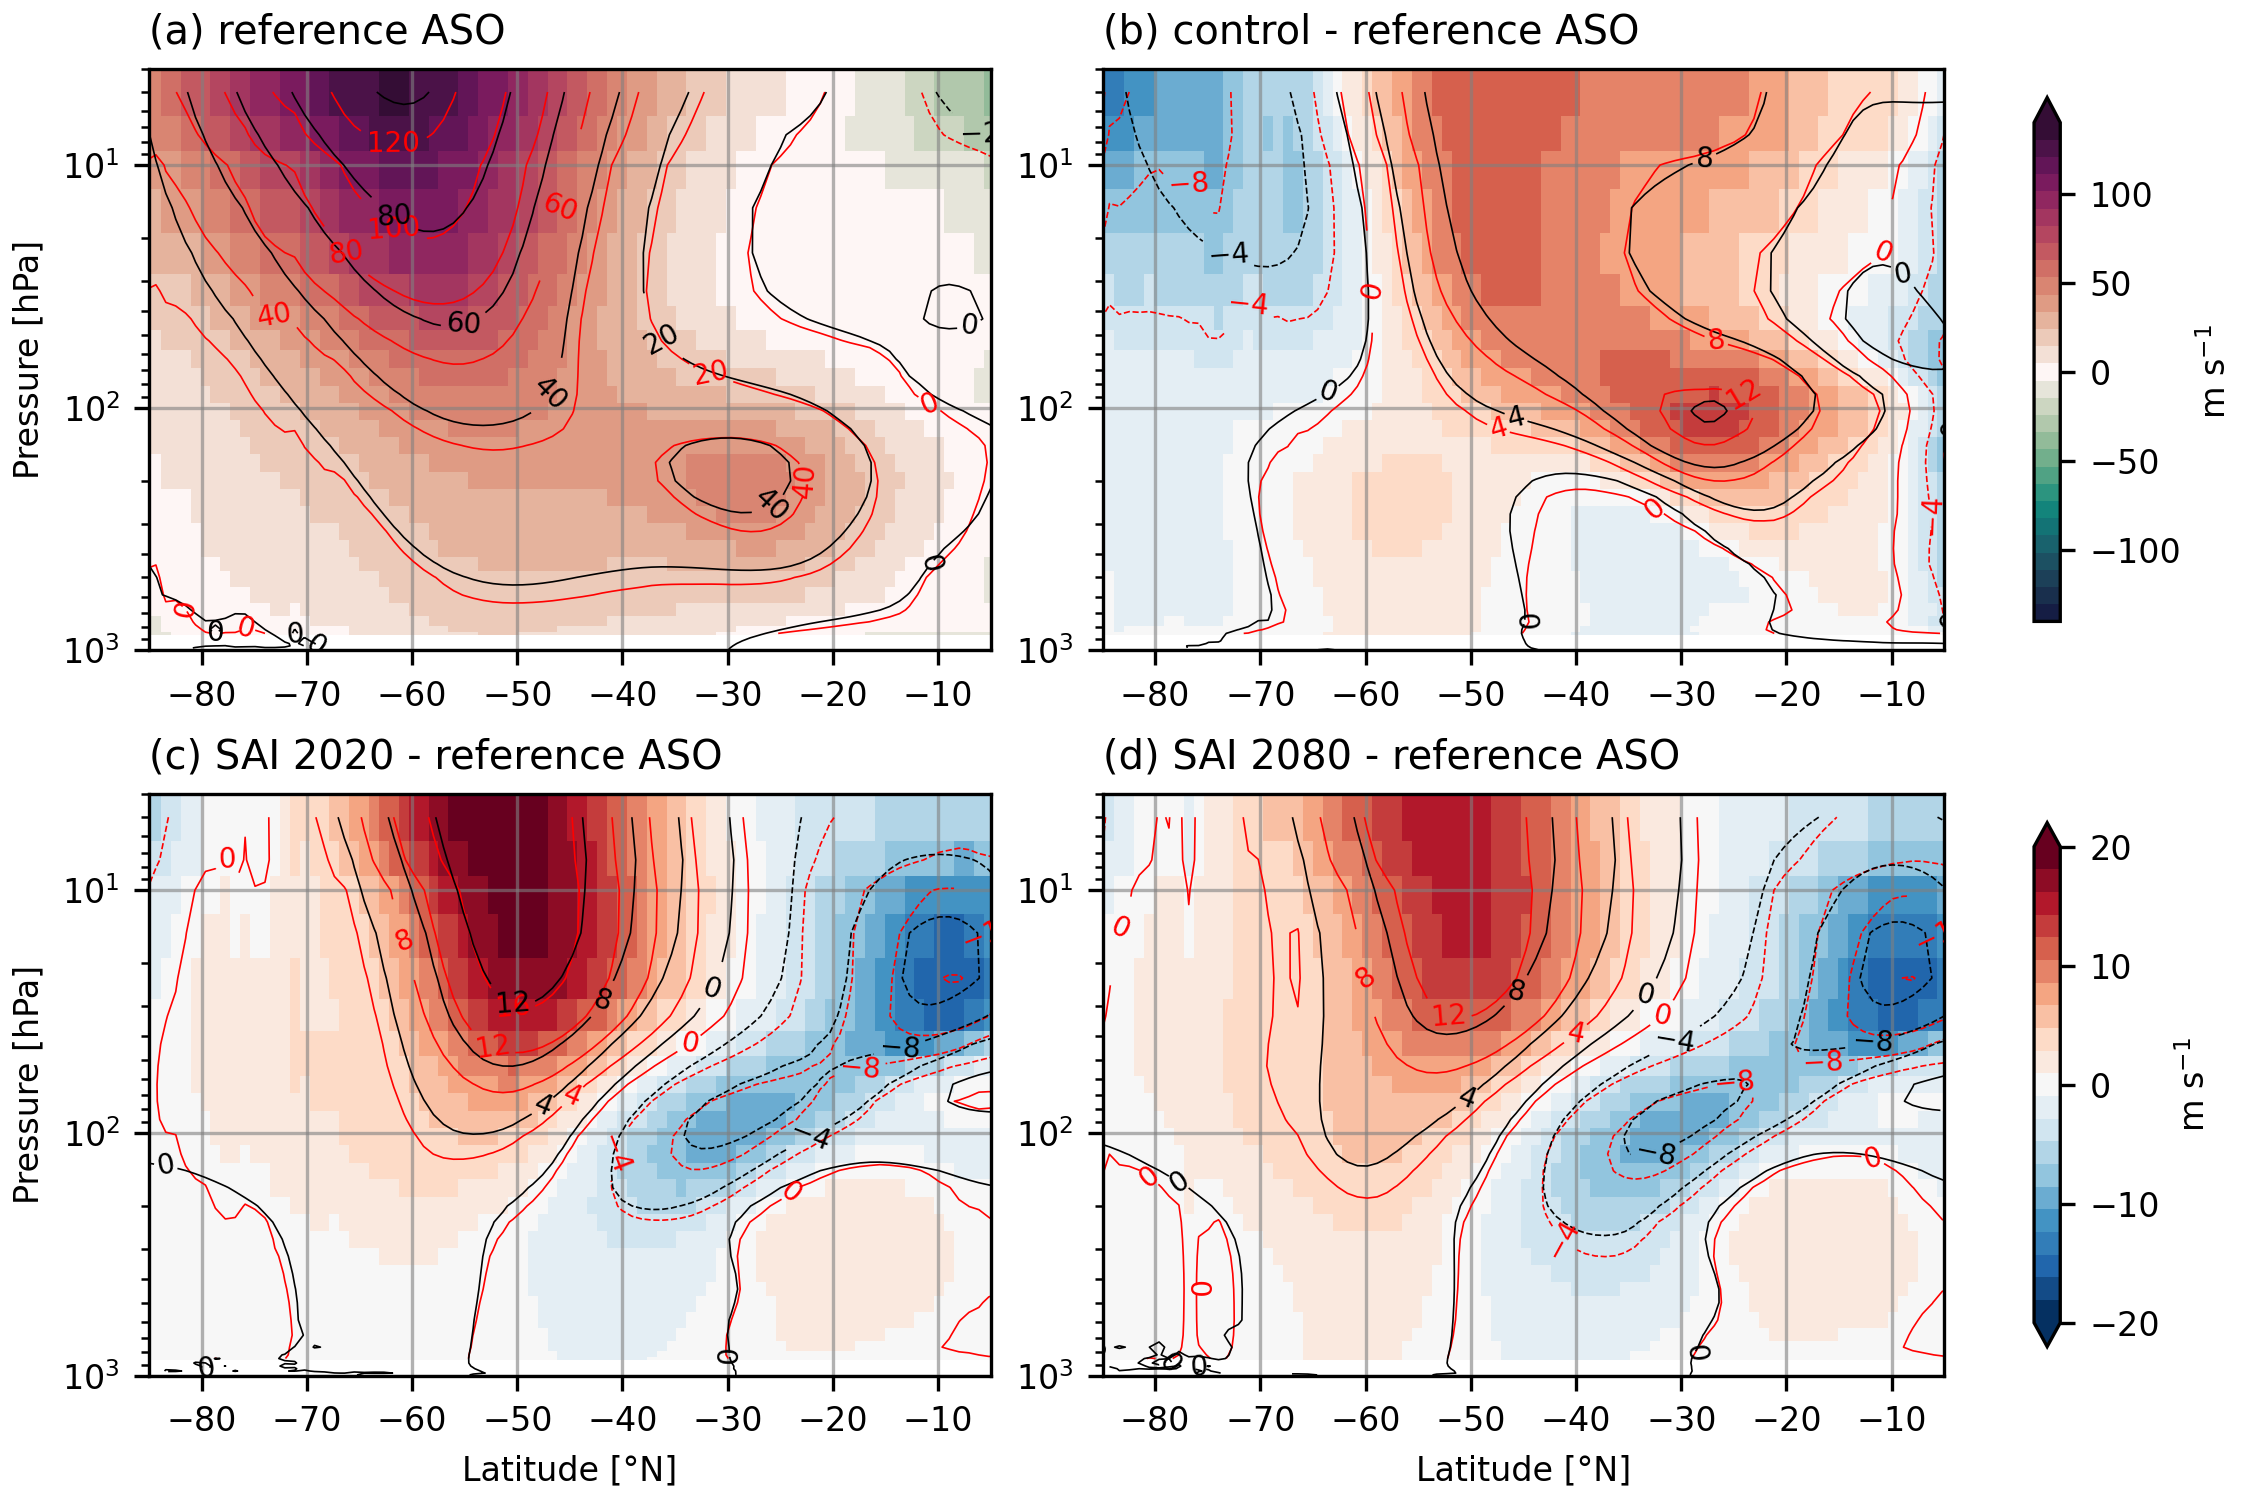
\includegraphics[width=0.95\linewidth]{images/PNJ_UT_U_zmdiff.png}
	\caption{ASO mean zonal mean kinetic energy (shading) and zonal mean zonal wind (contours) for (a): Reference; (b-d): Control, SAI 2020 and SAI 2080 anomaly compared to Reference.}
	\label{fig:PNJ_UT_U_zmdiff}
\end{figure}

\begin{figure}[H]
	\centering
	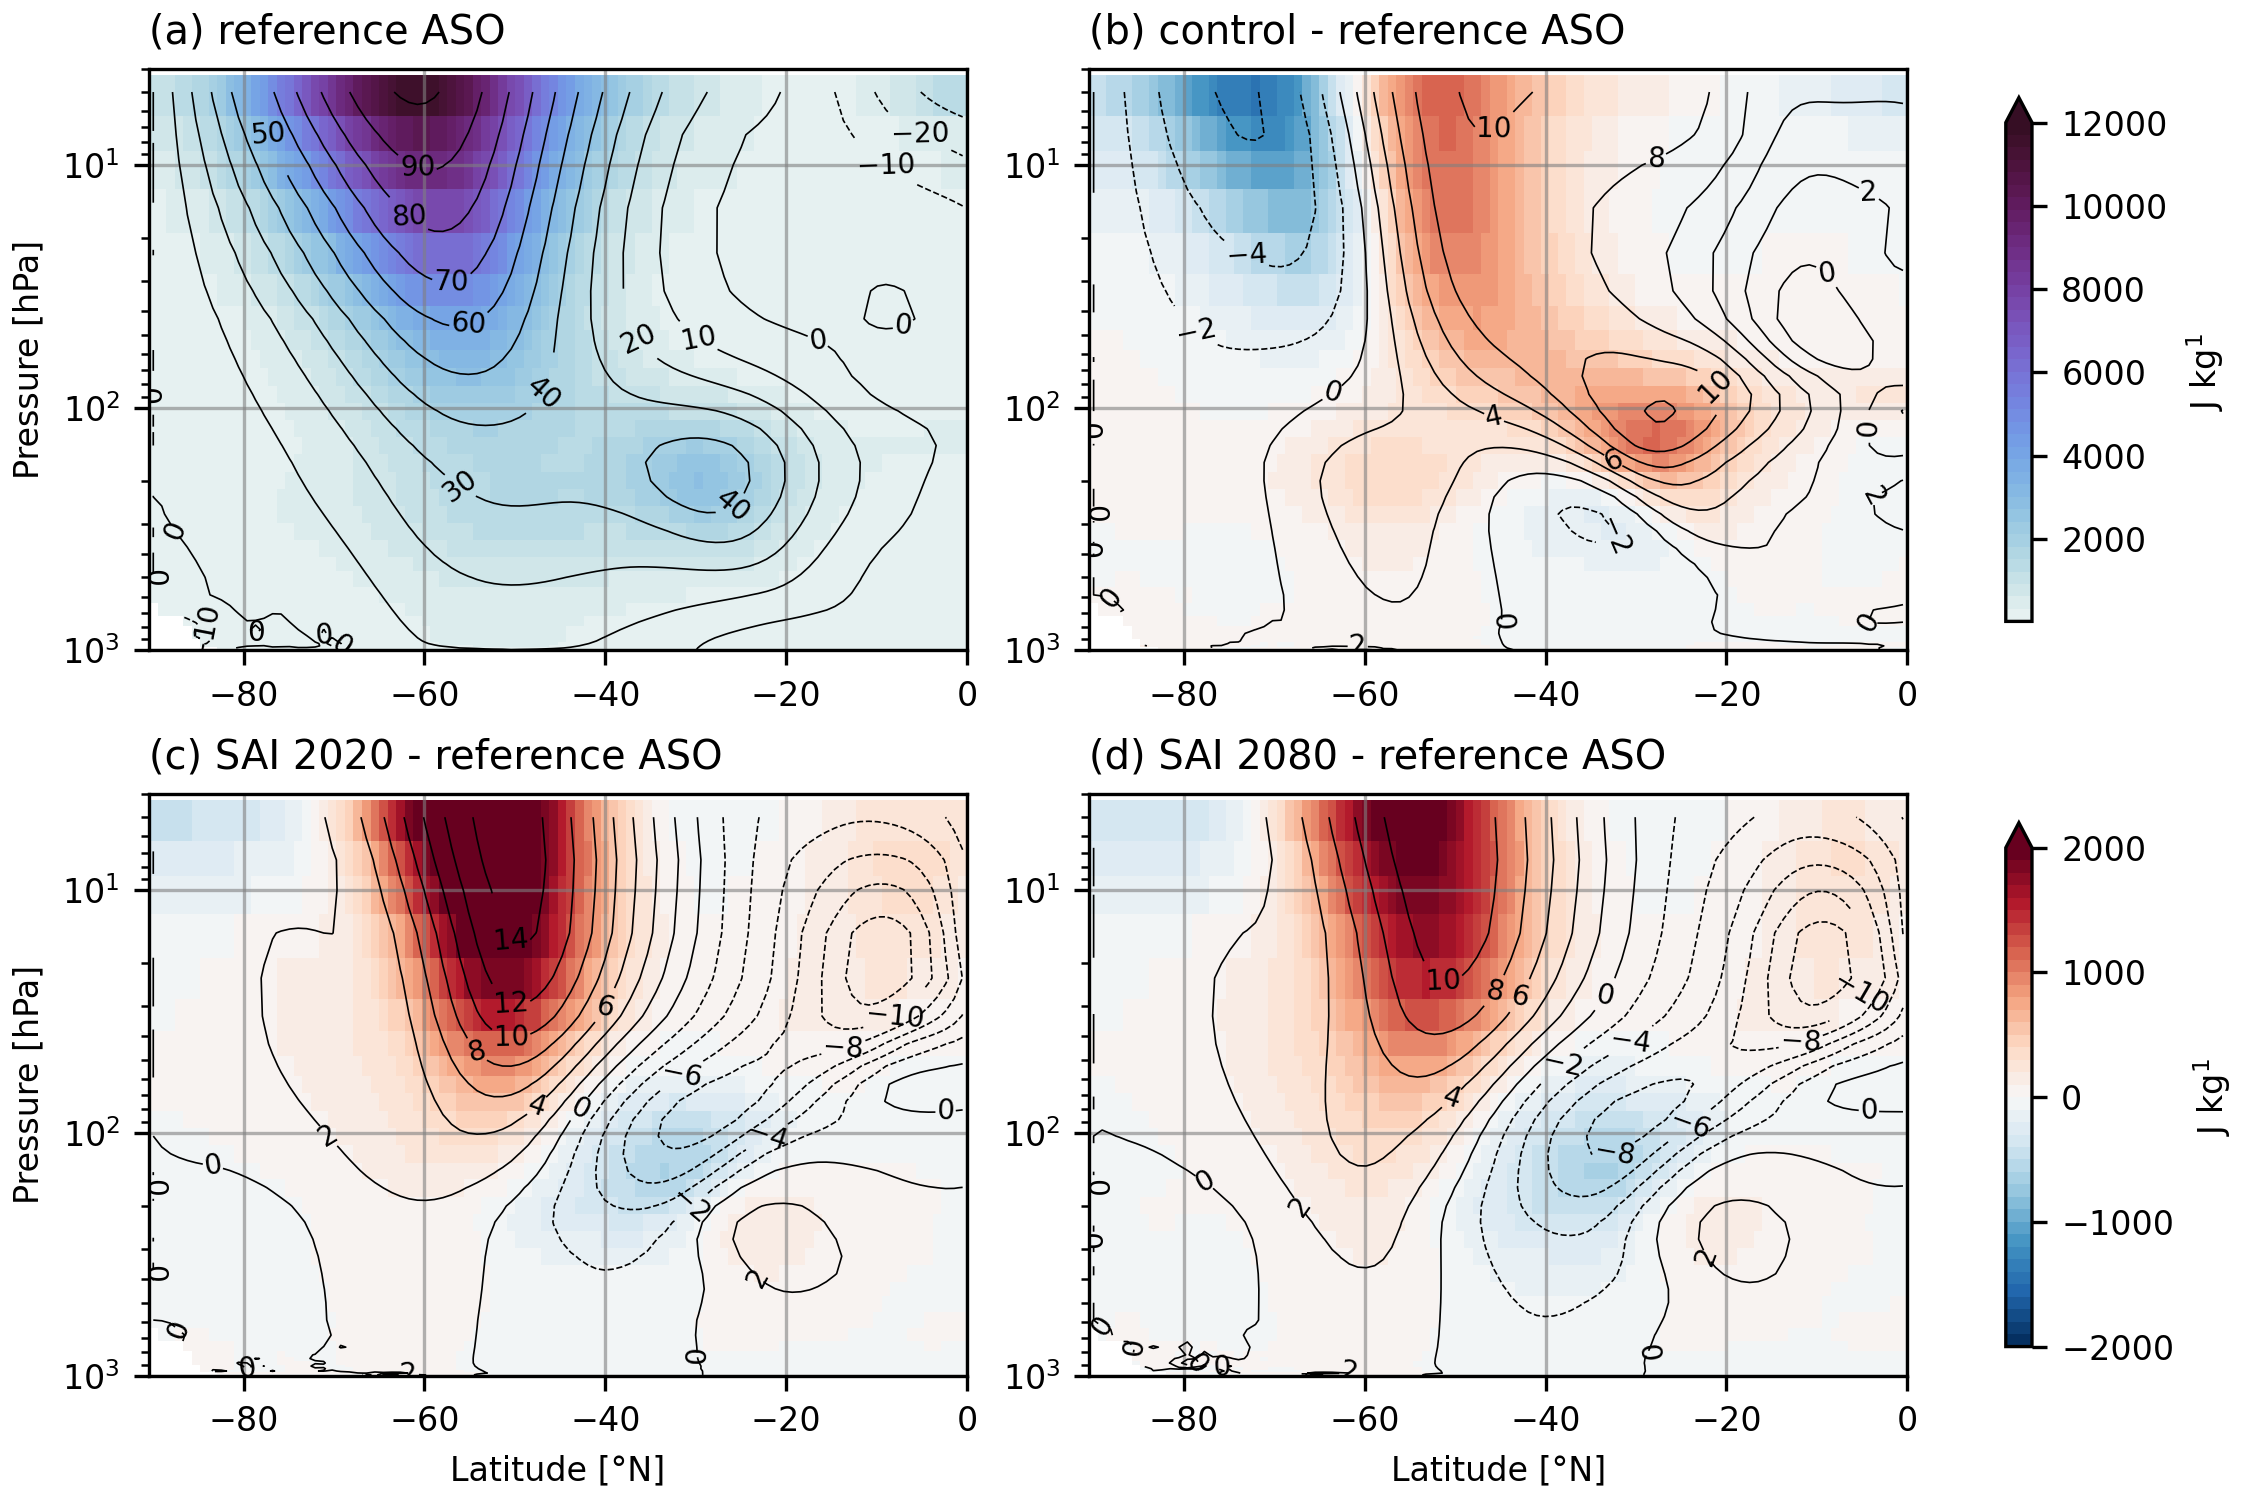
\includegraphics[width=0.95\linewidth]{images/PNJ_KE_U_zmdiff.png}
	\caption{JJA mean zonal mean eddy kinetic energy (shading) and zonal mean zonal wind (contours) for (a): Reference; (b-d): Control, SAI 2020 and SAI 2080 anomaly compared to Reference.}
	\label{fig:PNJ_KE_U_zmdiff}
\end{figure}


\begin{figure}[H]
	\centering
	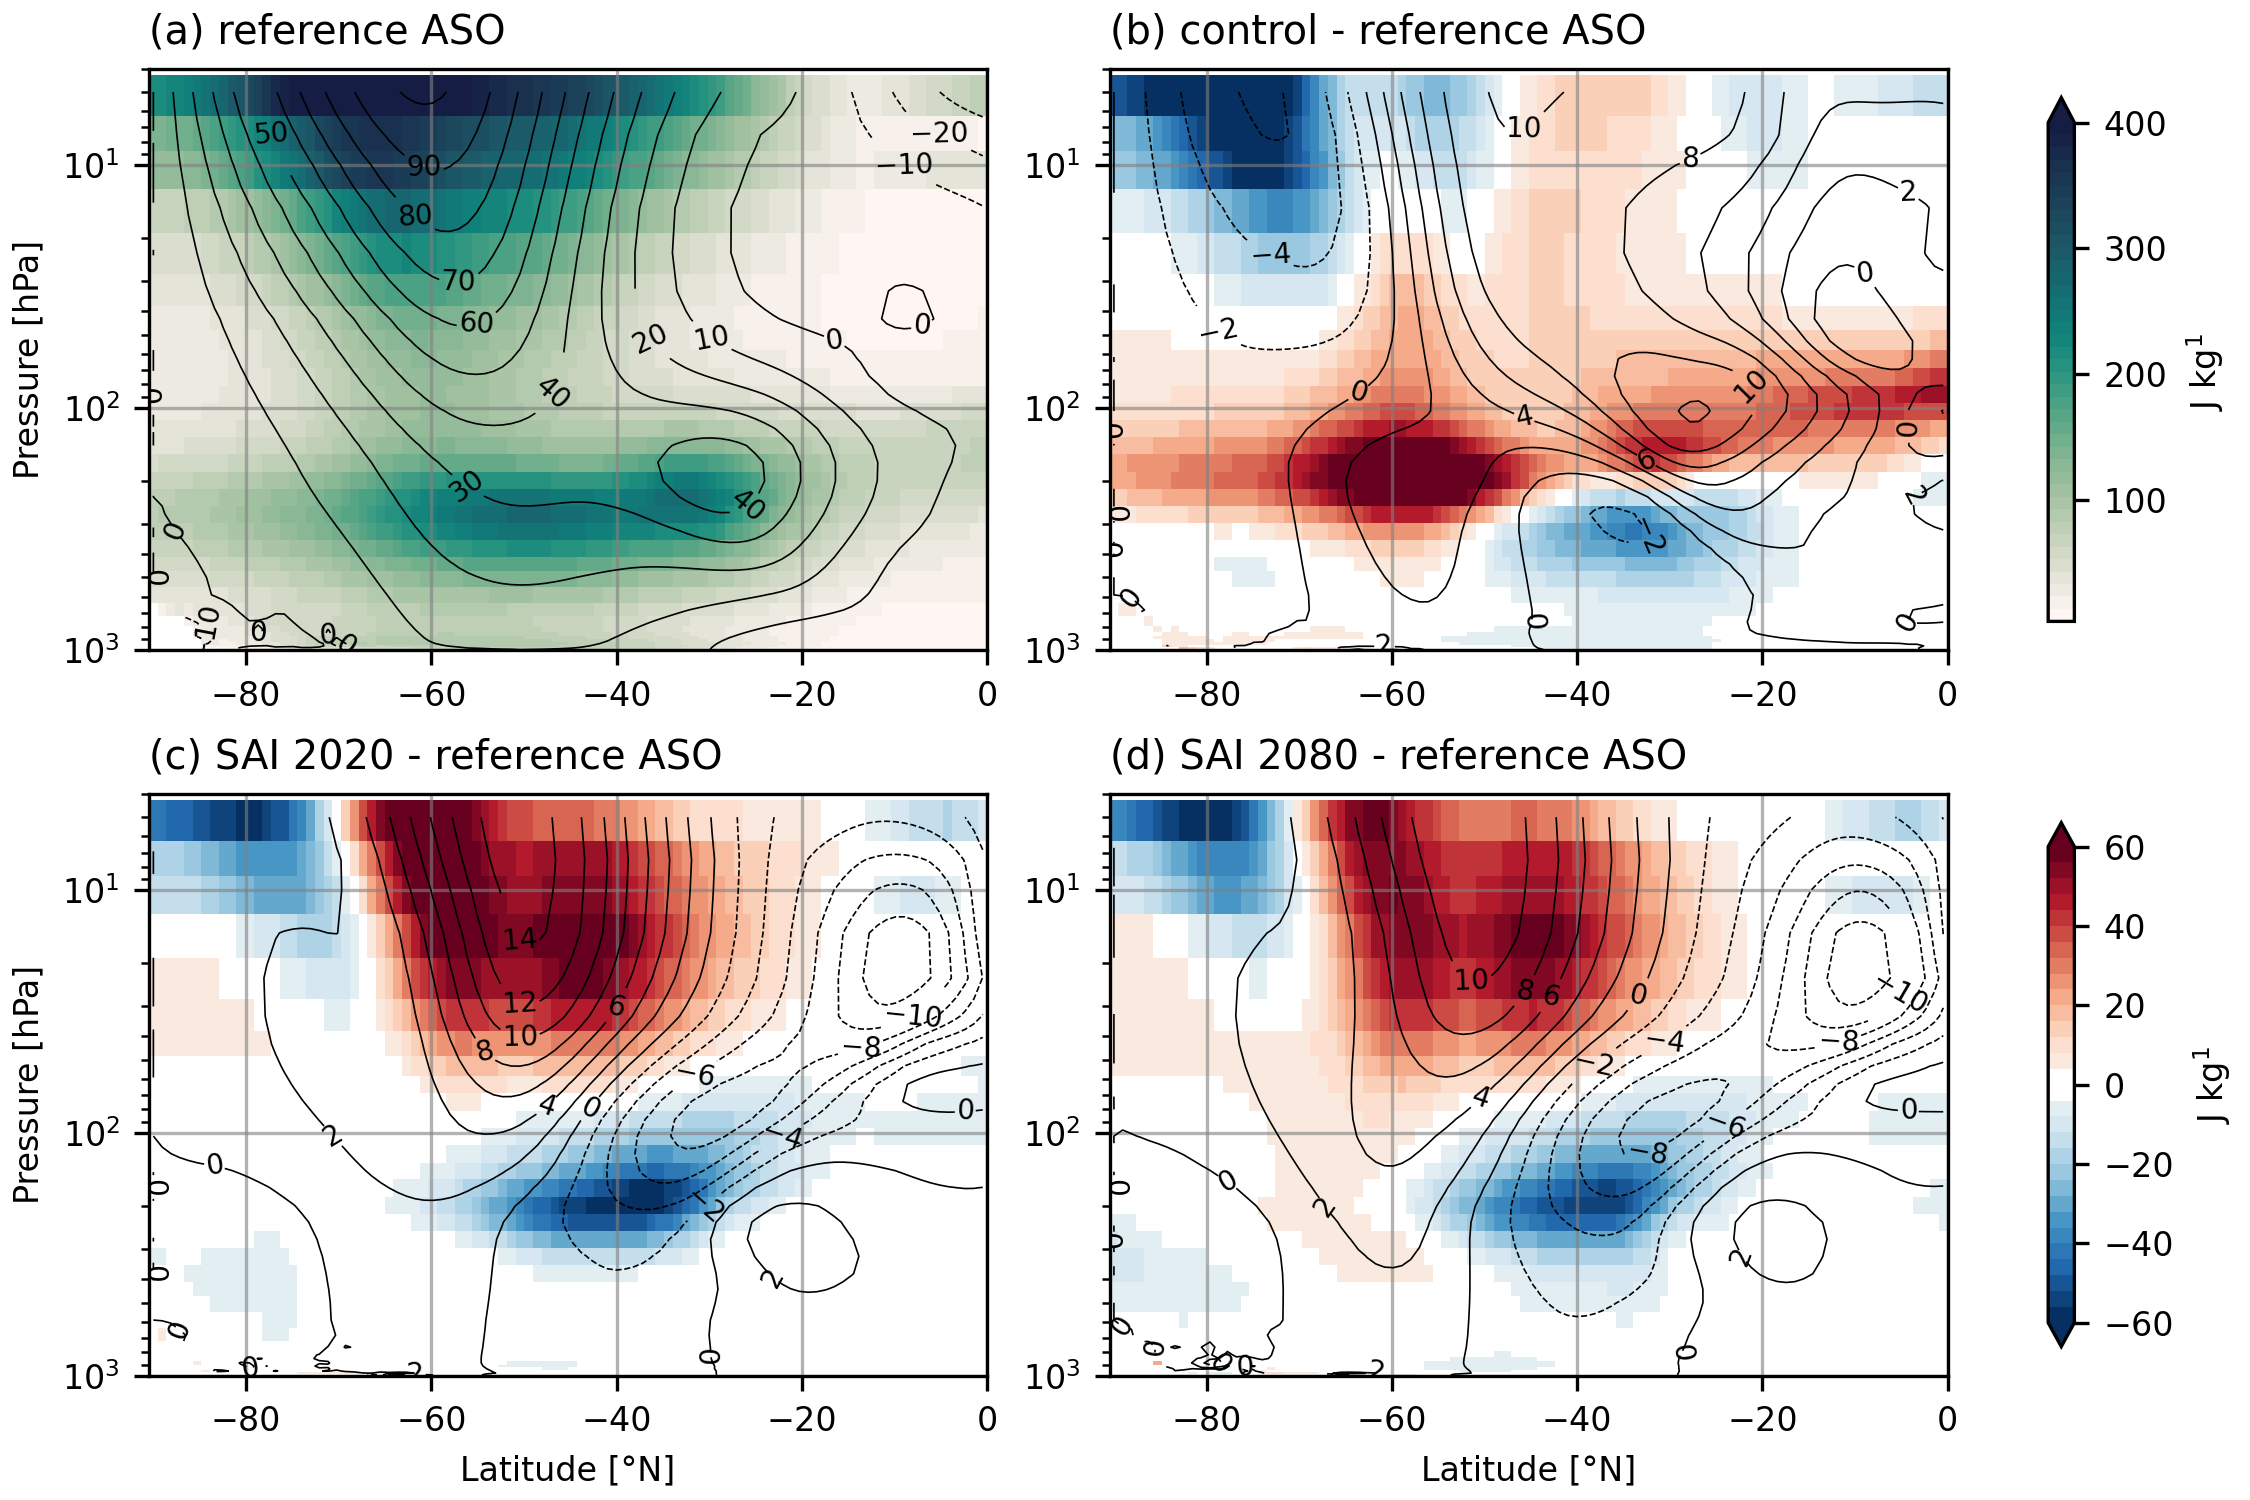
\includegraphics[width=0.95\linewidth]{images/PNJ_EKE_U_zmdiff.png}
	\caption{JJA mean zonal mean eddy kinetic energy (shading) and zonal mean zonal wind (contours) for (a): Reference; (b-d): Control, SAI 2020 and SAI 2080 anomaly compared to Reference.}
	\label{fig:PNJ_EKE_U_zmdiff}
\end{figure}

The increasing strength of the PNJ is again visible in the polar night jet intensity map in Figure \ref{fig:PNJ_map}. The PNJ intensifies in all scenarios, most strongly in SAI 2020, followed by SAI 2080 and lastly Control. The same trend is observed for the position, with the PNJ shifting equatorward in all scenarios. This equatorward shift is more clearly observed in Figure \ref{fig:PNJ_maxloc}, where the mean location of the maximum observed wind speed is shown. The scenario with the largest shift varies per location, with hardly any movement in any scenario in the 0°-60°E section, Control shifting the most in the 120°-180°E section, and SAI 2020 shifting the most in the 240°-300°E section. The shift in SAI 2080 is mostly consistent with SAI 2020, but deviates in the 240°-300°E section, coinciding with Control there.

\begin{figure}[H]
	\centering
	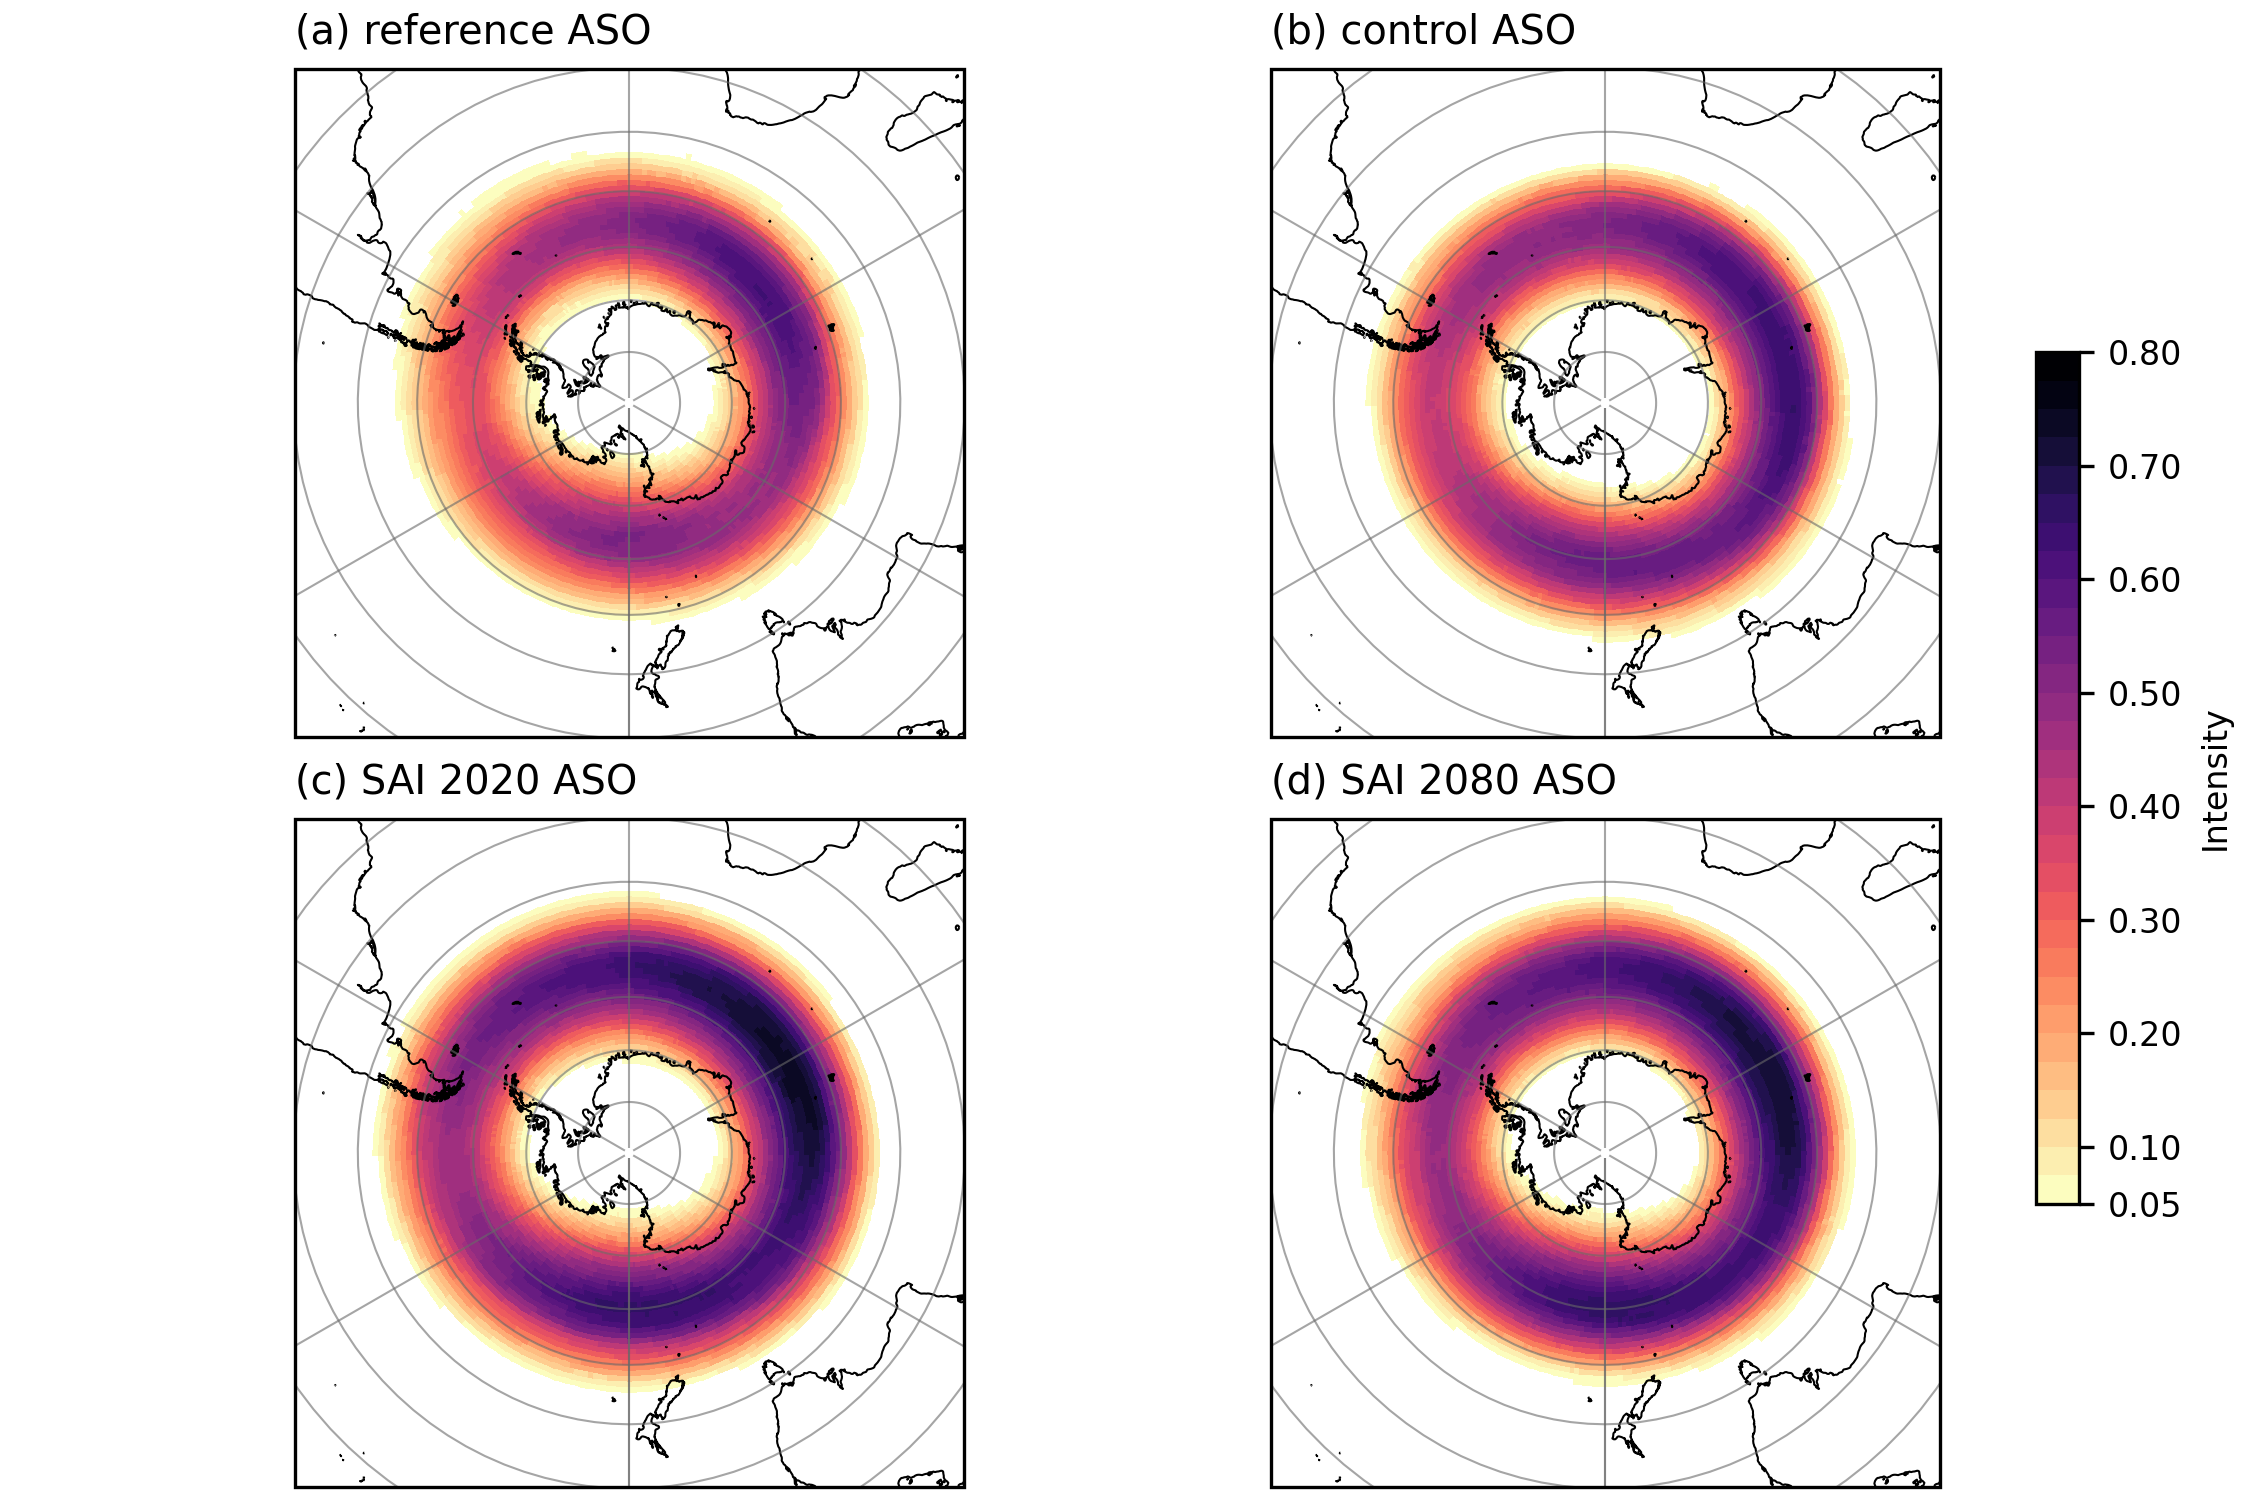
\includegraphics[width=0.95\linewidth]{images/PNJ_map.png}
	\caption{Polar night jet intensity map for (a) Reference, (b) Control, (c) SAI 2020 and (d) SAI 2080.}
	\label{fig:PNJ_map}
\end{figure}


\begin{figure}[H]
	\centering
	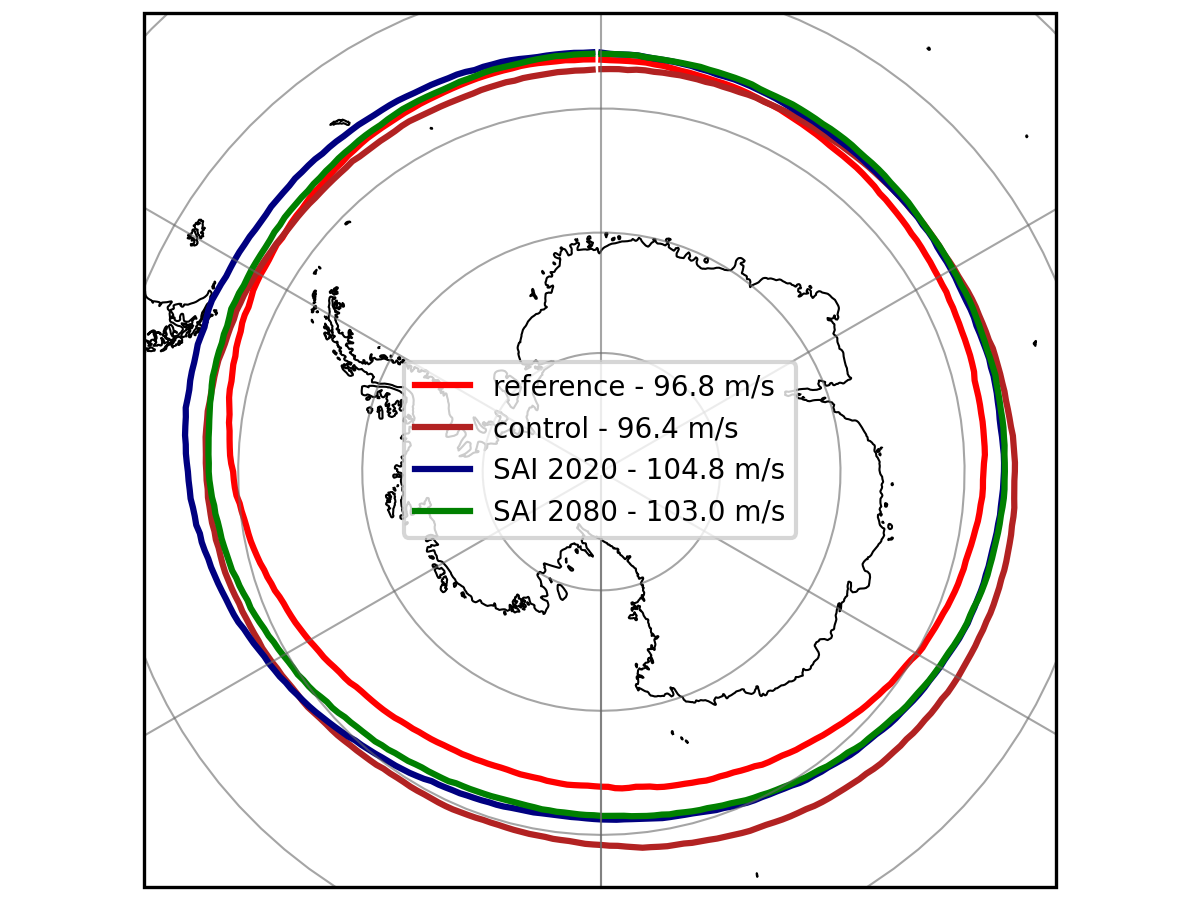
\includegraphics[width=0.48\linewidth]{images/PNJ_maxloc_latlon.png}
	\caption{Mean location of maximum wind speed at 10 hPa, with longitudinal mean maximum wind speed, for Reference, Control, SAI 2020 and SAI 2080.}
	\label{fig:PNJ_maxloc}
\end{figure}

\subsection{Sudden Stratospheric Warming Events}
The decrease in EKE over the Antarctic observed in \ref{fig:PNJ_EKE_U_zmdiff} suggests a decrease in the occurence of sudden stratospheric warming events (SSW). Figure \ref{fig:PNJ_climographTU} shows the area weighted mean temperature of the 10 hPa level above 60°S, together with the zonal wind at 10 hPa and 60°S. Note the  In Reference there is a number of years where the temperature increases and the zonal wind decreases compared to the mean. This indicates large scale SSW, as they are large enough, either in magnitude or duration, to show up in the monthly mean data. In Control the frequency of SSW-like conditions decreases significantly, the temperature and zonal wind bands narrow compared to Reference. In SAI 2020 there appears to be one year with SSW-like conditions, but again the temperature and zonal wind bands narrow. SAI 2080 shows the same trend. 

In all scenarios the zonal wind increases, as was already discussed in the results above, and the temperature decrease due to increased greenhouse gases is also visible. In all scenarios the PNJ forms earlier in the year, surpassing 75 m/s in early June in Control and late May in SAI 2020 and SAI 2080, as opposed to late June in Reference. The PNJ also dissolves later in the year, decreasing to 75 m/s in November in all scenarios as opposed to October in Reference.

\begin{figure}[H]
	\centering
	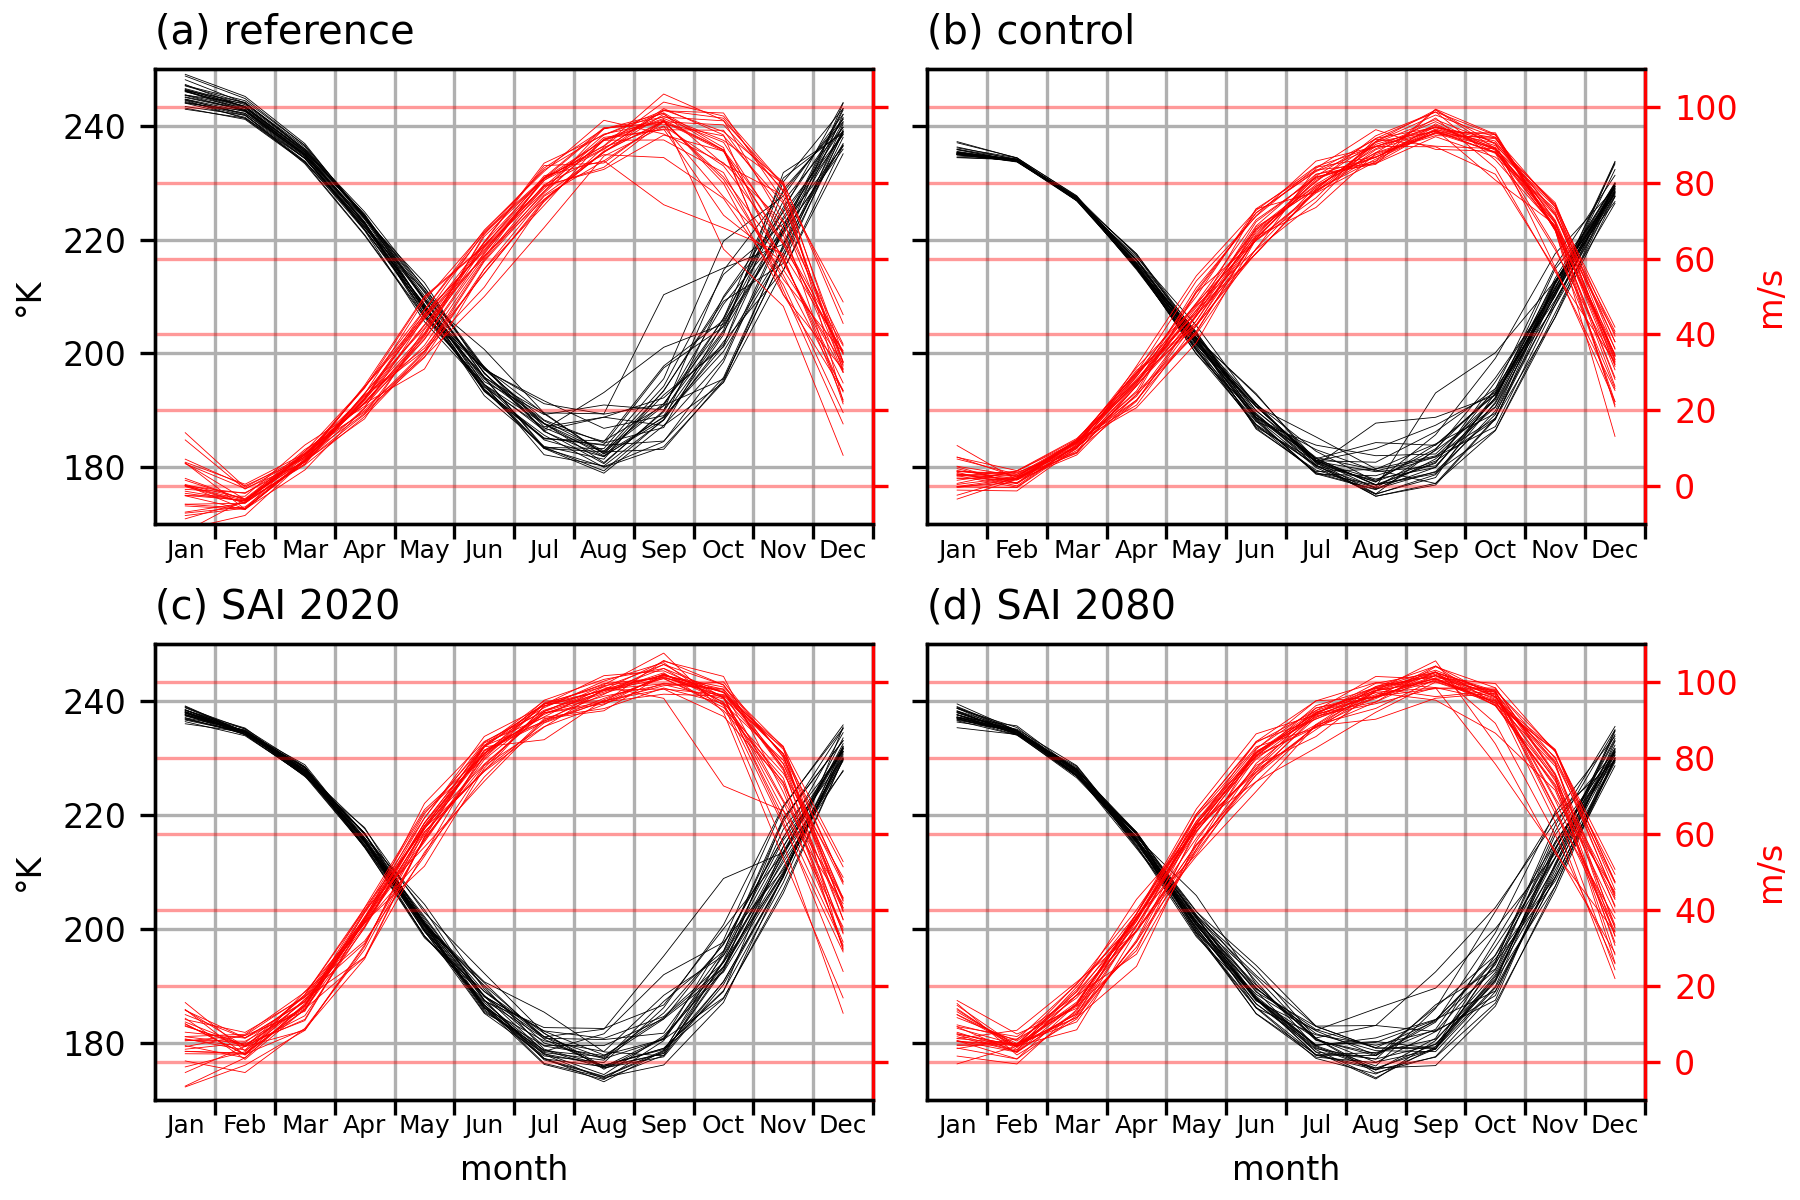
\includegraphics[width=0.95\linewidth]{images/PNJ_climographTU.png}
	\caption{Climograph of area-weighted mean temperature of 60°-90°S at 10 hPa (black) and zonal mean zonal wind at 60°S and 10 hPa (red) for (a) 2016-2045 and (b) 2101-2130 in the SSP5-8.5 experiment, (c) 2101-2130 in the gradual SAI experiment and (d) 2101-2130 in the rapid cooling SAI experiment.}
	\label{fig:PNJ_climographTU}
\end{figure}